\documentclass[class=minimal, border = 0pt, crop]{standalone}
\usepackage{pgf}
\usepackage{tikz}
\usepackage[utf8]{inputenc}
\usepackage{amsmath}
\usepackage{amsthm}
\DeclareMathAlphabet\mathbb{U}{msb}{m}{n}
\usetikzlibrary{arrows,automata,shapes,calc,backgrounds,decorations.pathreplacing}
\usetikzlibrary{decorations.pathmorphing}
\usetikzlibrary{positioning}
\pagestyle{empty}
\tikzset{
    state/.style={
           rectangle,
           rounded corners,
           draw=black, very thick,
           minimum height=2em,
           inner sep=5pt,
           text centered,
           },
    pil/.style={
           ->,
           thick,
           shorten <=4pt,
           shorten >=4pt,
           },
    ball/.style={
           circle,
           draw,
           align=center,
           anchor=north,
           inner sep=0,
           fill=black,
           }
}
\tikzset{discont/.style={decoration={zigzag,segment length=0.5cm, amplitude=0.25cm},decorate}}
\begin{document}
\centering
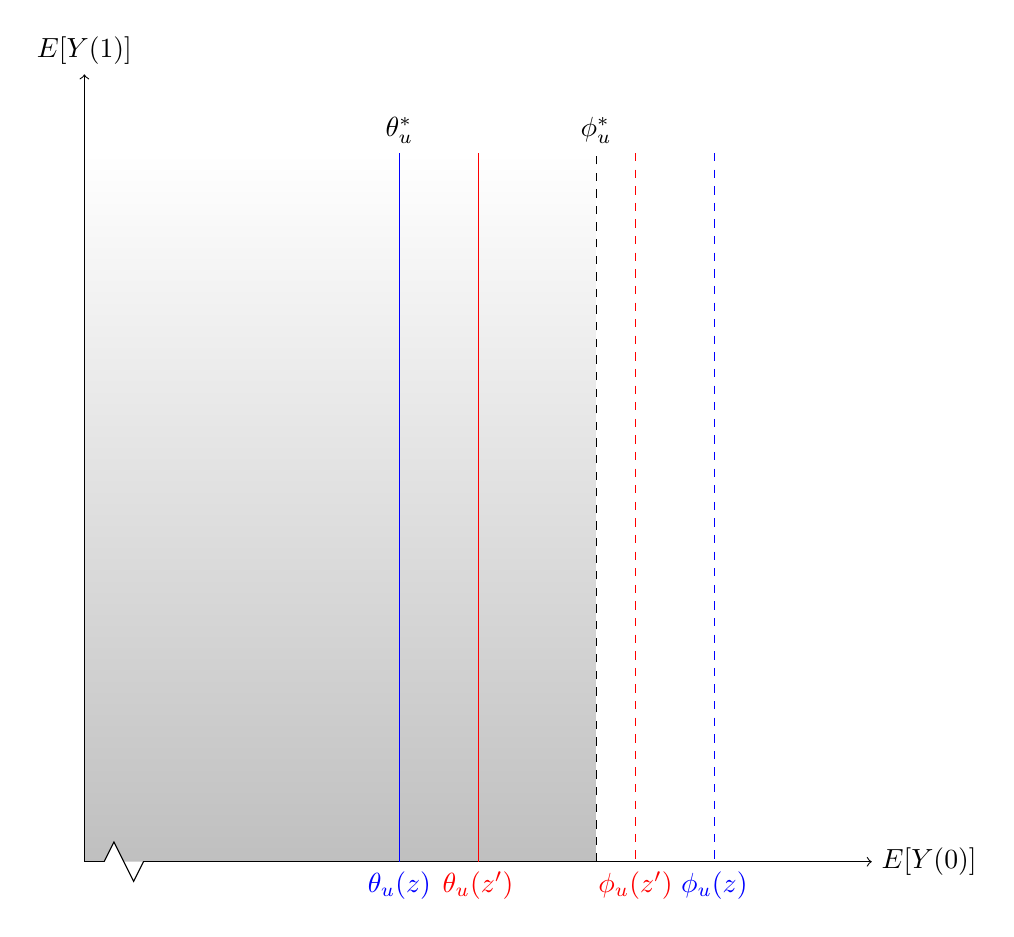
\begin{tikzpicture}
 \coordinate (O) at (0,0);
 \begin{scope}
 \clip (0.25,0) -- (0.375,0.25) -- (0.5,0) -- (6.5,0) -- (6.5,10) -- (0,10) -- (0,0) -- cycle;
 \shadedraw [top color=white,bottom color=gray!50,draw=none] (0,0) rectangle (6.5,9);
 \end{scope}
 \draw (0,0) -- (0.25,0); 
 \draw[discont] (0.25,0) -- (0.75,0);
 \draw[->] (0,0) -- (0,10) coordinate[label = {above:$\mathbb{E}[Y(1)]$}] (ymax);
 \draw[->] (0.75,0) -- (10,0) coordinate[label = {right:$\mathbb{E}[Y(0)]$}] (xmax);
 \draw[color=black,draw=none] (4,0) -- (4,9) coordinate[label = {above:$\theta_u^*$}] (ymin);
 \draw[color=blue] (4,9) -- (4,0) coordinate[label = {below:$\theta_u(z)$}] (ymin);
 \draw[color=blue,dashed] (8,9) -- (8,0) coordinate[label = {below:$\phi_u(z)$}] (ymin);
 \draw[color=red] (5,9) -- (5,0) coordinate[label = {below:$\theta_u(z')$}] (ymin);
 \draw[color=red,dashed] (7,9) -- (7,0) coordinate[label = {below:$\phi_u(z')$}];
 \draw[dashed] (6.5,0) -- (6.5,9)  coordinate[label = {above:$\phi_u^*$}];
\end{tikzpicture}
\end{document}